% article example for classicthesis.sty
\documentclass[10pt,a4paper]{article} % KOMA-Script article scrartcl
\usepackage{import}
\usepackage{xifthen}
\usepackage{pdfpages}
\usepackage{transparent}
\newcommand{\incfig}[1]{%
    \def\svgwidth{\columnwidth}
    \import{./figures/}{#1.pdf_tex}
}
\usepackage{lipsum}     %lorem ipsum text
\usepackage{titlesec}   %Section settings
\usepackage{titling}    %Title settings
\usepackage[margin=10em]{geometry}  %Adjusting margins
\usepackage{setspace}
\usepackage{listings}
\usepackage{amsmath}    %Display equations options
\usepackage{amssymb}    %More symbols
\usepackage{xcolor}     %Color settings
\usepackage{pagecolor}
\usepackage{mdframed}
\usepackage[spanish]{babel}
\usepackage[utf8]{inputenc}
\usepackage{longtable}
\usepackage{multicol}
\usepackage{graphicx}
\graphicspath{ {./Images/} }
\setlength{\columnsep}{1cm}

% ====| color de la pagina y del fondo |==== %
\pagecolor{black}
\color{white}



\begin{document}
    %========================{TITLE}====================%
    \title{{  Apuntes clase 4 vectores de medias y matrices de covarianza  }}
    \author{{Rodrigo Castillo}}
    \date{\today}

    \maketitle


     % ====| Loguito |==== %
    
\includegraphics[width=0.1\linewidth]{negro_cara.png}
    %=======================NOTES GOES HERE===================%
    \section{Vectores y matrices aleatorios}
        definicones :
        \\ vector aleatorio: \color{red} vector cuyos elementos son variables
        aleatorias \color{white}
        \\ Matriz aleatoria : \color{red} matriz cuyos elementos son variables
        aleatorias \color{white}
        \\ valor esperado de una matriz aleatoria : \color{red} el valor
        esperado de una matriz aleatoria es la matriz de los valores esperados
        de cada uno de sus elementos \color{white}

        \begin{figure}[h!]
            \centering
            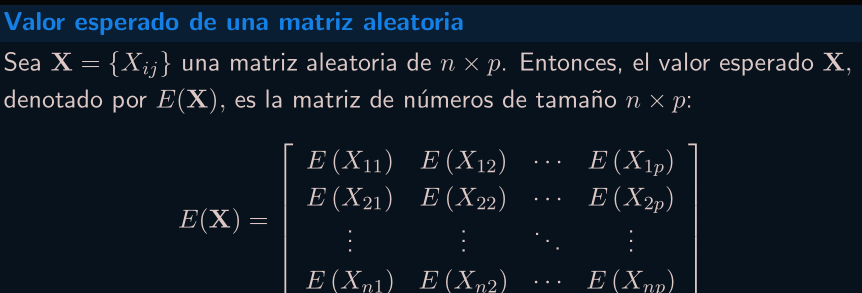
\includegraphics[width=0.8\linewidth]{valesp.png}
            \caption{valor esperado de una matriz}
            \label{fig:valesp}
        \end{figure}

        donde cada elemento es ...

        \begin{figure}[h!]
            \centering
            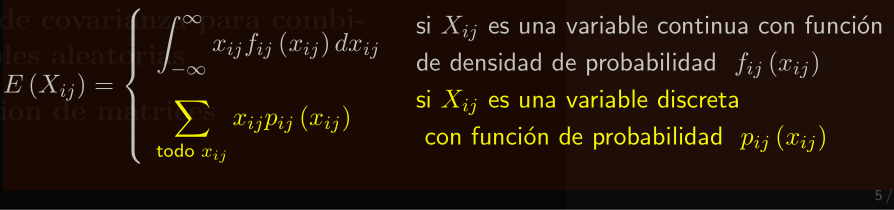
\includegraphics[width=0.8\linewidth]{valesp2.png}
            \caption{Valesp2}
            \label{fig:valesp2}
        \end{figure}

        \newpage
        valor esperado de sumas y productos de matrices ...
        \begin{equation}
            \color{red} E(X+Y) = E(X) + E(Y) \color{white}
        \end{equation}
        \begin{equation}
            \color{red} E(AXB) =  AE(X)B \color{white}
        \end{equation}



    \section{Vectores de media y matrices de covarianza}
    \section{particion de la matriz de covarianza}
    \section{vector de media y matriz de covarianza para combinaciones lineales de variables aleatorias}
    \section{Desigualdaes y maximizacion de matrices}
    \section{Dudas}








    %=======================NOTES ENDS HERE===================%

    % bib stuff
    \nocite{*}
    \addtocontents{toc}{{}}
    \addcontentsline{toc}{section}{\refname}
    \bibliographystyle{plain}
    \bibliography{../Bibliography}
\end{document}
